\part{Maxwell's theory}

\chapter{Maxwell's action}

    In this chapter, we will review some notion of classical electrodynamics: Maxwell's Lagrangian that leads to the Maxwell's equations and how, using gauge symmetry in vacuum, an electromagnetic wave carries only two degrees of freedom, which are the two transversal polarisations indepependent components.

\section{Maxwell's Lagrangian}

    Classical free electrodynamic fields, without sources, can be describe starting from the Maxwell's Lagrangian
    \begin{equation}\label{maxlag}
    \begin{aligned}
        \mathcal L & = - \frac{1}{4} F_{\mu\nu} F^{\mu\nu} = - \frac{1}{4} (\partial_\mu A_\nu - \partial_\nu A_\mu) (\partial^\mu A^\nu - \partial^\nu A^\mu) \\ & = - \frac{1}{4} ( \partial_\mu A_\nu \partial^\mu A^\nu - \partial_\nu A_\mu \partial^\mu A^\nu - \partial_\mu A_\nu \partial^\nu A^\mu + \partial_\nu A_\mu  \partial^\nu A^\mu ) \\ & = - \frac{1}{2} (\partial_\mu A_\nu \partial^\mu A^\nu - \partial_\nu A_\mu \partial^\mu A^\nu) ~,
    \end{aligned}
    \end{equation}
    where $F_{\mu\nu}$ is the electromagnetic tensor
    \begin{equation*}
        F_{\mu\nu} = \partial_\mu A_\nu - \partial_\nu A_\mu = \begin{bmatrix}
            0 & E_1 & E_2 & E_3 \\ 
            -E_1 & 0 & - B_3 & B_2 \\ 
            - E_2 & B_3 & 0 & - B_1 \\ 
            - E_3 & -B_2 & B_1 & 0 \\
        \end{bmatrix}
    \end{equation*}
    and the $4$-potential is $A^\mu = (\phi, \mathbf A)$. Recall that they are related to the electric and the magnetic field via 
    \begin{equation}\label{ef}
        \mathbf B = \boldsymbol \nabla \times \mathbf A ~, \quad \mathbf E = - \boldsymbol \nabla \phi - \pdv{\mathbf A}{t} 
    \end{equation}
    and we can write them in terms of the electromagnetic tensor as 
    \begin{equation*}
        E_i = F_{0i} ~, \quad B_i = \frac{1}{2} \epsilon_{ijk} F^{jk} ~.
    \end{equation*}
    From this Lagrangian, we recover the equation of motion, which are exactly Maxwell's equations in vacuum
    \begin{equation*}
        \partial_\mu F^{\mu\nu} = 0 ~.
    \end{equation*}
    \begin{proof}
        Using~\eqref{eleq} and~\eqref{maxlag}, we have
        \begin{equation*}
        \begin{aligned}
            0 & = \partial_\mu \pdv{\mathcal L}{\partial_\mu A_\nu} - \underbrace{\pdv{\mathcal L}{A_\nu}}_0 = \partial_\mu \pdv{}{\partial_\mu A_\nu} (- \frac{1}{2} (\partial_\alpha A_\beta \partial^\alpha A^\beta - \partial_\beta A_\alpha \partial^\alpha A^\beta)) \\ & = - \partial_\mu (\partial^\mu A^\nu - \partial^\nu A^\nu) = - \partial_\mu F^{\mu\nu} ~.
        \end{aligned}
        \end{equation*}
    \end{proof}
    An useful property of the electromagnetic tensor is that it satisfies the Bianchi identity 
    \begin{equation*}
        \partial_\mu F_{\nu\lambda} + \partial_\nu F_{\lambda \mu} + \partial_\lambda F_{\mu \nu} = 0 ~.
    \end{equation*}
    \begin{proof}
        In fact, we have 
        \begin{equation*}
        \begin{aligned}
            \partial_\mu F_{\nu\lambda} + \partial_\nu F_{\lambda \mu} + \partial_\lambda F_{\mu \nu} & = \partial_\mu (\partial_\nu A_\lambda - \partial_\lambda A_\nu) + \partial_\nu (\partial_\lambda A_\mu - \partial_\mu A_\lambda) + \partial_\lambda (\partial_\mu A_\nu - \partial_\nu A_\mu) \\ & = \partial_\mu \partial_\nu A_\lambda -  \partial_\mu \partial_\lambda A_\nu + \partial_\nu \partial_\lambda A_\mu - \partial_\nu  \partial_\mu A_\lambda + \partial_\lambda \partial_\mu A_\nu - \partial_\lambda \partial_\nu A_\mu \\ & = \cancel{\partial_\nu \partial_\mu A_\lambda} - \cancel{\partial_\lambda \partial_\mu A_\nu} +  \cancel{\partial_\lambda \partial_\nu A_\mu} - \cancel{\partial_\nu \partial_\mu A_\lambda} + \cancel{\partial_\lambda \partial_\mu A_\nu} - \cancel{\partial_\lambda \partial_\nu A_\mu} = 0 ~,
        \end{aligned}
        \end{equation*}
        where we have used the fact that partial derivatives commute.
    \end{proof}
    We define the dual electromagnetic tensor
    \begin{equation*}
        \tilde F^{\mu\nu} = - \frac{1}{2} \epsilon^{\mu\nu\rho\sigma} F_{\rho\sigma} ~,
    \end{equation*}
    or, explicitly, 
    \begin{equation*}
        \tilde F_{\mu\nu} = \begin{bmatrix}
            0 & - B_1 & - B_2 & - B_3 \\ 
            B_1 & 0 & E_3 & -E_2 \\ 
            B_2 & -E_3 & 0 & E_1 \\ 
            B_3 & E_2 & -E_1 & 0 \\
        \end{bmatrix} ~.
    \end{equation*}
    Notice that there is a duality symmetry, since if we perfom the exhange $\mathbf E \leftrightarrow - \mathbf B$, we find $F^{\mu\nu} \leftrightarrow \tilde F^{\mu\nu}$. We can write the Bianchi identity in terms of the dual tensor as
    \begin{equation*}
        \partial_\mu \tilde F^{\mu\nu} = - \frac{1}{2} \epsilon^{\mu\nu\rho\sigma} \partial_\mu  F_{\rho\sigma} = 0 ~.
    \end{equation*}
    \begin{proof}
        In fact, we have
        \begin{equation*}
        \begin{aligned}
            0 & = \partial_\mu F_{\nu\lambda} + \partial_\nu F_{\lambda \mu} + \partial_\lambda F_{\mu \nu} = \epsilon^{\mu\nu\lambda\sigma} (\partial_\mu F_{\nu\lambda} + \partial_\nu F_{\lambda \mu} + \partial_\lambda F_{\mu \nu}) \\ & = \partial_\mu \epsilon^{\mu\nu\lambda\sigma} F_{\nu\lambda} + \partial_\nu \epsilon^{\mu\nu\lambda\sigma} F_{\lambda \mu} + \partial_\lambda \epsilon^{\mu\nu\lambda\sigma} F_{\mu \nu} = \cancel{\partial_\mu \epsilon^{\sigma\mu\nu\lambda} F_{\nu\lambda}} - \cancel{\partial_\nu \epsilon^{\sigma\nu\lambda\mu} F_{\lambda\mu}} + \partial_\lambda \epsilon^{\lambda\sigma\mu\nu} F_{\mu \nu} \\ & = \epsilon^{\mu\nu\rho\sigma} \partial_\mu  F_{\rho\sigma} ~.
        \end{aligned}
        \end{equation*}
    \end{proof}

    It can be proved that the Maxwell's equations in covariant formalism can be written as 
    \begin{equation*}
        \boldsymbol \nabla \cdot \mathbf B = 0 ~, \quad \pdv{\mathbf B}{t} = - \boldsymbol \nabla \times \mathbf E \quad \Rightarrow \quad \partial_\mu \tilde F^{\mu\nu} = 0 ~,
    \end{equation*}
    \begin{equation*}
        \boldsymbol \nabla \cdot \mathbf E = 0 ~, \quad \pdv{\mathbf E}{t} = \boldsymbol \nabla \times \mathbf E \quad \Rightarrow \quad \partial_\mu F^{\mu\nu} = 0 ~.
    \end{equation*}
    In presence of sources, the first one remains the same whereas the second one changes because it carries information about them. 

\section{Gauge symmetry}

    It is useful to rewrite the Maxwell's Lagrangian in terms of temporal and spatial indices
    \begin{equation*}
        \mathcal L = - \frac{1}{2} (F_{0i} F^{0i} + F_{ij} F^{ij} ) ~.
    \end{equation*} 
    \begin{proof}
        In fact, we have 
        \begin{equation*}
        \begin{aligned}
            \mathcal L & = - \frac{1}{4} (\partial_\mu A_\nu - \partial_\nu A_\mu)(\partial^\mu A^\nu - \partial^\nu A^\mu) \\ & = -\frac{1}{4} (\partial_\mu A_\nu \partial^\mu A^\nu - \partial_\mu A_\nu \partial^\nu A^\mu -  \partial_\nu A_\mu \partial^\mu A^\nu + \partial_\nu A_\mu \partial^\nu A^\mu) \\ & = - \frac{1}{2} (\partial_\mu \partial^\mu A^\nu A_\nu - \partial_\nu \partial^\mu A^\nu A_\mu) \\ & = - \frac{1}{2} (\cancel{\partial_0 \partial^0 A^0 A_0} + \partial_0 \partial^0 A^i A_i + \partial_i \partial^i A^0 A_0 + \partial_i \partial^i A^j A_j \\ & \quad - \cancel{\partial_0 \partial^0 A^0 A_0} - \partial_0 \partial^i A^0 A_i - \partial_i \partial^j A^i A_j - \partial_i \partial^0 A^i A_0) \\ & = - \frac{1}{2} (\partial_0 \partial^0 A^i A_i + \partial_i \partial^i A^0 A_0 + \partial_i \partial^i A^j A_j - \partial_0 \partial^i A^0 A_i - \partial_i \partial^j A^i A_j - \partial_i \partial^0 A^i A_0) \\ & = - \frac{1}{2} 
            (\partial_0 \partial^0 A^i A_i - \partial_0 \partial^i A_i A^0 - \partial_i  \partial^0 A^0 A^i + \partial_j \partial^j A_i A^i \\ & \quad - \partial_i \partial^j A_j A^i + \partial_j \partial^i A_i A^j + \partial_i \partial^j A_j A^i - \partial_i \partial^i A_j A^j ) \\ & = - \frac{1}{2} ((\partial_0 A_i - \partial_i A_0) (\partial^0 A^i - \partial^i A^0) - (\partial_j A_i - \partial_i A_j) (\partial^j A^i - \partial^i A^j)) \\ & = - \frac{1}{2} (F_{0i} F^{0i} + F_{ij} F^{ij} ) ~.
        \end{aligned}
        \end{equation*}
    \end{proof}
    Notice that there is no dependence on the kinetic part of $A^0$, i.e. $\dot A^0$, which means that $A^0$ is fully determined by $A^i$. Therefore, we do not need to specify initial condition for $A_0$ at $t=t_0$ since the ones of $A_i$ and $\dot A_i$ are sufficient, and $A_\mu$ seems to contain only $3$ independent components. This is a consequence of the Gauss' law, which implies that
    \begin{equation*}
        A_0 (t_0, \mathbf x) = \int d^3 y ~ \frac{1}{4\pi |\mathbf x - \mathbf y} \boldsymbol \nabla \cdot \pdv{\mathbf A}{t} (t_0, \mathbf y)  ~.
    \end{equation*}
    \begin{proof}
        Using the Gauss' law, we have 
        \begin{equation*}
            0 = - \boldsymbol \nabla \cdot \mathbf E = \boldsymbol \nabla \cdot \boldsymbol \nabla A_0 + \boldsymbol \nabla \cdot \pdv{\mathbf A}{t} ~,
        \end{equation*}
        \begin{equation*}
            \nabla^2 A_0 (t_0, \mathbf x) = \boldsymbol \nabla \cdot \pdv{\mathbf A}{t} (t_0, \mathbf x) ~.
        \end{equation*}
        Now, we use the Green function to solve this differential equation. The Green operator is 
        \begin{equation*}
            \nabla^2 G (t_0, \mathbf x - \mathbf y) = \delta^3 (\mathbf x - \mathbf y) ~.
        \end{equation*}
        By a Fourier transform 
        \begin{equation*}
            G (t_0, \mathbf x - \mathbf y) = \int \frac{d^3 p}{(2\pi)^3} ~ \tilde G (p) \exp(- i \mathbf p \cdot (\mathbf x - \mathbf y)) ~,
        \end{equation*}
        we find 
        \begin{equation*}
        \begin{aligned}
            \nabla^2_x G (t_0, \mathbf x - \mathbf y) & = \nabla^2_x \int \frac{d^3 p}{(2\pi)^3} ~ \tilde G (p) \exp(- i \mathbf p \cdot (\mathbf x - \mathbf y)) \\ &= \int \frac{d^3 p}{(2\pi)^3} ~ \tilde G (p) (- p^2) \exp(- i \mathbf p \cdot (\mathbf x - \mathbf y)) \\ & = \delta^3 (\mathbf x - \mathbf y) = \int \frac{d^3 p}{(2\pi)^3} ~ \exp(- i \mathbf p \cdot (\mathbf x - \mathbf y)) ~.
        \end{aligned}
        \end{equation*}
        which implies that 
        \begin{equation*}
            \tilde G (p) = - \frac{1}{p^2} ~.
        \end{equation*}
        Putting inside the Fourier transform and using polar coordinates in momentum space, we obtain 
        \begin{equation*}
        \begin{aligned}
            G (t_0, \mathbf x - \mathbf y) & = - \int \frac{d^3 p}{(2\pi)^3} ~ \frac{\exp(- i \mathbf p \cdot (\mathbf x - \mathbf y))}{p^2} \\ & = - 2 \pi \frac{1}{(2\pi)^3} \int_0^\infty dp ~ p^2 \int_0^\pi d\theta ~ \sin \theta \frac{\exp(- i p \cos\theta |\mathbf x - \mathbf y|)}{p^2} \\ & = - \frac{1}{4 \pi^2} \int_0^\infty dp \int_{-1}^{1} d (- \cos \theta) ~ \exp(- i p \cos \theta |\mathbf x - \mathbf y|) \\ & = - \frac{1}{4 \pi^2} \int_0^\infty dp ~ \frac{\exp(-i p \cos \theta |\mathbf x - \mathbf y|)}{i p |\mathbf x - \mathbf y|} \Big \vert_{-\cos \theta = -1}^{-\cos \theta = 1} \\ & = - \frac{1}{4 \pi^2 |\mathbf x - \mathbf y| i} \int_0^\infty dp ~ \frac{\exp(i p \cos \theta |\mathbf x - \mathbf y|)}{p} - \frac{\exp(-i p \cos \theta |\mathbf x - \mathbf y|)}{p} \\ & = - \frac{1}{4 \pi^2 |\mathbf x - \mathbf y| i} \int_{-\infty}^\infty dp ~ \frac{\exp(i p \cos \theta |\mathbf x - \mathbf y|)}{p}  \\ & = - \frac{1}{4 \pi^2 |\mathbf x - \mathbf y| i} \pi i \exp (i p |\mathbf x - \mathbf y|) \Big \vert_{p = 0} = - \frac{1}{4 \pi |\mathbf x - \mathbf y|} ~,
        \end{aligned}
        \end{equation*}
        where we have integrated in the upper-part of the complex plane with one pole in $p=0$. Finally, we find 
        \begin{equation*}
            A_0 (t_0, \mathbf x) = - \int d^3 y ~ G(\mathbf x - \mathbf y) \boldsymbol \nabla \cdot \pdv{\mathbf A}{t} (t_0, \mathbf y) = \int d^3 y ~ \frac{1}{4\pi |\mathbf x - \mathbf y|} \boldsymbol \nabla \cdot \pdv{\mathbf A}{t} (t_0, \mathbf y)~.
        \end{equation*}
    \end{proof}

    This is a signal that Maxwell's theory is a gauge theory. In fact, Maxwell's Lagrangian is symmetric with respect to a gauge transformation  
    \begin{equation*}
        {A'}_\mu (x) = A_\mu (x) + \partial_\mu \alpha (x) ~,
    \end{equation*}
    where $\alpha (x)$ is an arbitrary gauge function of spacetime coordinates, such that its derivative vanishes at spatial infinity.
    \begin{proof}
        In fact, we have
        \begin{equation*}
            {F'}^{\mu\nu} = \partial_\mu {A'}_\nu - \partial_\nu {A'}_\mu = \partial_\mu A_\nu - \partial_\nu A_\mu + \cancel{\partial_\mu \partial_\nu \alpha(x)} - \cancel{\partial_\nu \partial_\mu \alpha(x)} = \partial_\mu A_\nu - \partial_\nu A_\mu = F^{\mu\nu} ~,
        \end{equation*}
        which means that
        \begin{equation*}
            \mathcal L' = - \frac{1}{4} {F'}^{\mu\nu} F'_{\mu\nu} = - \frac{1}{4} F^{\mu\nu}_{\mu\nu} = \mathcal L ~.
        \end{equation*}
    \end{proof}

    However, we experimentally know that an electromagnetic wave traveling in vacuum has only two degrees of freedom corresponding to the two transversal polarisations. This signals that there is a second residual gauge transformation 
    \begin{equation*}
        {A''}_\mu (x) = {A'}_\mu (x) + \partial_\mu \beta (x) = A_\mu (x) + \partial_\mu (\alpha (x) + \beta (x) ) ~,
    \end{equation*}
    where $\beta (x)$ is the second gauge function. Physically, $A$, $A'$ and $A''$ descibe the same physical state, since the Lagrangians are the same. Therefore, they define a class of equivalence of physical points of view. There are several choices for the representative of this class or gauge orbit by some conditions, called gauge fixing, based on the convenience to make easier the problem. See Figure~\ref{fig:gauge}. It is important to highlight the difference between a global and a local symmetry. A global symmetry does not depend on the spacetime coordinates and it is a true symmetry of the system, which leads to the Noether's theorem. A local symmetry is just a redundancy in the description of the physics and it does not have a conservation law (even because there will be infinitely many).

    \begin{figure}[h!]
        \centering
        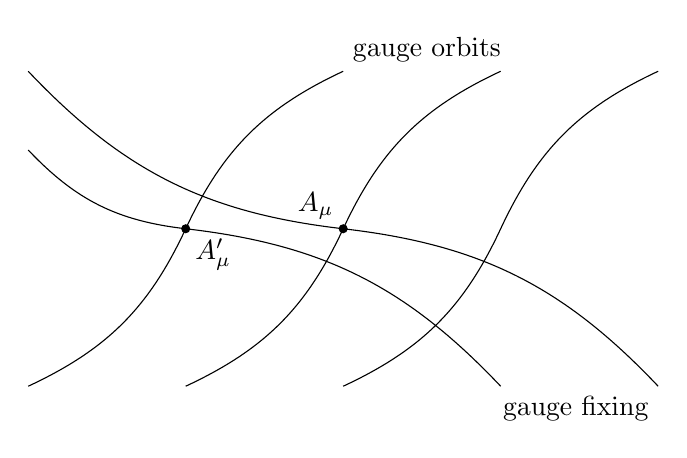
\begin{tikzpicture}
        \draw[] (0,0) to[bend right=20] (2,2) to[bend left=20] (4,4) node[above right] {gauge orbits};
        \draw[] (2,0) to[bend right=20] (4,2) to[bend left=20] (6,4) ;
        \draw[] (4,0) to[bend right=20] (6,2) to[bend left=20] (8,4) ;

        \draw[] (0,4) to[bend right=20] (4,2) to[bend left=20] (8,0) node[below left] {gauge fixing};
        \draw[] (0,3) to[bend right=20]  (2,2) to[bend left=20] (6,0) ;

        \filldraw[black] (4,2) circle (0.05) node[above left] {$A_\mu$};
        \filldraw[black] (2,2) circle (0.05) node[below right] {$A'_\mu$};

        \end{tikzpicture}
        \caption{Pictorial representation of gauge orbits and gauge fixing.}
        \label{fig:gauge}
    \end{figure}
    
    The gauge fixing we will use in this notes is the Lorenz gauge, which is manifestly Lorentz invariant and brings down the number of degrees of freedom to $2$
    \begin{equation*}
        \partial_\mu A^\mu = 0 ~.
    \end{equation*}
    \begin{proof}
        With a gauge transformation, we have
        \begin{equation*}
            {A'}_\mu (x) = A_\mu (x) + \partial_\mu \alpha (x) ~,
        \end{equation*}
        where $\alpha (x)$ must satisfy 
        \begin{equation*}
            0 = \partial_\mu {A'}^\mu = \partial_\mu A^\mu + \Box \alpha (x) ~,
        \end{equation*}
        hence, we find
        \begin{equation*}
            \Box \alpha(x) = \partial_\mu A^\mu ~.
        \end{equation*}
        With the second gauge transformation, we have
        \begin{equation*}
            {A''}_\mu (x) = {A'}_\mu (x) + \partial_\mu \beta (x) ~,
        \end{equation*}
        where $\beta (x)$ must satisfy 
        \begin{equation*}
            \partial_\mu {A''}^\mu = \partial_\mu {A'}^\mu + \Box \beta (x) ~,
        \end{equation*}
        hence, we find
        \begin{equation*}
            \Box \beta(x) = 0 ~.
        \end{equation*}
    \end{proof}
    The equations of motion in the Lorenz gauge become 
    \begin{equation}\label{lgem}
        \Box A^\mu (x) = 0 ~.
    \end{equation}
    Notice that the Maxwell's equations in the Lorentz gauge are equal to the Klein-Gordon ones with mass equals to zero. This ensures that the mass shell condition is preserved. This means that each components of $A^\mu$ separately satisfies the mass shell condition. At quantum level, we will see taht $A_\mu$ describes particles (photons) with energy $E_{\mathbf p} = |\mathbf p|$.
    \begin{proof}
        In fact, we have
        \begin{equation*}
            0 = \partial_\mu F^{\mu\nu} = \partial_\mu (\partial^\mu A^\nu - \partial^\nu A^\mu) = \Box A^\nu - \partial^\nu \underbrace{\partial_\mu A^\mu}_0 = \Box A^\nu ~.
        \end{equation*}
    \end{proof}

    The conjugate momentum of $A_\mu$ is 
    \begin{equation*}
        \pi^\mu = (0, \mathbf E) ~.
    \end{equation*}
    \begin{proof}
        In fact, for $\mu = 0$, we have
        \begin{equation*}
            \pi^0 = \pdv{\mathcal L}{\dot A_0} = 0 ~,
        \end{equation*}
        whereas, for $\mu = i$, we have
        \begin{equation*}
        \begin{aligned}
            \pi^i = \pdv{\mathcal L}{\dot A_i} = - \frac{1}{2} \pdv{}{\dot A_i} ((\dot A_j - \partial_j A_0))(\dot A^j - \partial^j A_0) = - \frac{1}{2} \pdv{}{\dot A_i} (F_{0j} F^{0j}) = - F^{0i} = E^i ~.
        \end{aligned}
        \end{equation*}
    \end{proof}

    The Hamiltonian is 
    \begin{equation*}
        H = \int d^3 x ~\Big ( \frac{1}{2}  (|E|^2 + |B|^2) - A_0 (\boldsymbol \nabla \cdot \mathbf E) \Big) ~.
    \end{equation*}
    Notice that we have a Lagrange multiplier $A_0$ to ensure the constrain of the Gauss' law, since $A_0$ is not a physical variable. In fact, one of the Hamilton's equation is
    \begin{equation*}
        0 = \dot A_0 = \pdv{\mathcal H}{A_0} = - \boldsymbol \nabla \cdot \mathbf E ~. 
    \end{equation*}
    \begin{proof}
        In fact, by a Legendre transformation and~\eqref{ef}, we have
        \begin{equation*}
        \begin{aligned}
            \mathcal H & = \pi^\mu \dot A_\mu - \mathcal L = \pi^i \dot A_i - \mathcal L = - E^i \underbrace{\dot A_i}_{- E_i - \partial_i A_0} - \mathcal L \\ & = E^i E_i + E^i \partial_i A_0 - \frac{1}{2} (|E|^2 - |B|^2) = \frac{1}{2} (|E|^2 + |B|^2) + E^i \partial_i A_0 ~,
        \end{aligned}
        \end{equation*}
        hence, we find
        \begin{equation}
        \begin{aligned}
            H & = \int d^3 x ~ \mathcal H = \int d^3 x ~ \Big ( \frac{1}{2} (|E|^2 + |B|^2) + \underbrace{E^i \partial_i A_0}_{- A_0 \partial_i E^i + \textnormal{boundary terms}} \Big) \\ & = \int d^3 x ~ \Big ( \frac{1}{2} (|E|^2 + |B|^2) - A_0 (\boldsymbol \nabla \cdot \mathbf E) \Big) ~.
        \end{aligned}
        \end{equation}
    \end{proof}

\chapter{Quantisation}

    In this chapter, we will quantise the Maxwell's theory. We will find field operators by canonical commutation relations, we will analyse the Fock space, finding which are the physical states compatible with the Lorenz gauge, and we will find the Hamiltonian operator.

\section{Quantisation without Lorenz gauge}

    The first guess to quantise the theory is, instead of imposind by hand the Lorenz gauge, to modify the Lagrangian 
    \begin{equation*}
        \mathcal L = - \frac{1}{4} F_{\mu\nu} F^{\mu\nu} - \frac{1}{2} (\partial_\mu A^\mu)^2 ~. 
    \end{equation*}
    Therefore, the equations of motion remains the same, even if we do not impose the Lorenz gauge, and the conjugate momentum becomes
    \begin{equation*}
        \pi^\mu = (- \partial_\mu A^\mu, F^{i0}) = F^{\nu 0} - \eta^{\nu 0} \partial_\mu A^\mu ~.
    \end{equation*}
    \begin{proof}        
        For the equations of motion, using~\eqref{eleq}, we have 
        \begin{equation*}
            0 = \partial_\mu \pdv{\mathcal L}{\partial_\mu \partial_\mu A_\nu} = - \partial_\mu F^{\mu\nu} - \partial^\nu \partial_\alpha A^\alpha ~,
        \end{equation*}
        hence, we obtain 
        \begin{equation*}
            0 = \partial_\mu F^{\mu\nu} + \partial_\mu \eta^{\mu\nu} \partial_\alpha A^\alpha = \partial_\mu \partial^\mu A^\nu - \partial_\mu \partial^\nu A^\mu + \partial^\nu \partial_\alpha A^\alpha = \partial_\mu \partial^\mu A^\nu ~,
        \end{equation*}
        where we have used the fact that partial derivatives commute.
        For the conjugate momentum, for $\mu = 0$, we have
        \begin{equation*}
            \pi^0 = \pdv{\mathcal L}{\dot A_0} = - \frac{1}{2} \pdv{\mathcal L}{\dot A_0} (\partial_\mu A^\mu)^2 = - \partial_\mu A^\mu  ~,
        \end{equation*}
        whereas, for $\mu = i$, we have
        \begin{equation*}
            \pi^i = E^i = - F^{0i} = F^{i0} ~.
        \end{equation*}
        Finally, to recover the covariant formalism, we find
        \begin{equation*}
            \pi^0 = \underbrace{F^{00}}_0 - \underbrace{\eta^{00}}_1 (\partial_\mu A^\mu) = - \partial_\mu A^\mu 
        \end{equation*}
        and 
        \begin{equation*}
            \pi^i = F^{0i} - \underbrace{\eta^{i0}}_0 (\partial_\mu A^\mu) = F^{0i} ~.
        \end{equation*}
    \end{proof}

    Now, we use the machinery of second quantisation: in Schoedinger picture, we promote $A^\mu(x)$ and $\pi^\mu(x)$ to operators in the Fock space by imposing the canonical commutation, since we have an integer spin theory ($s = 1$), 
    \begin{equation*}
        [\hat A_\mu (\mathbf x), \hat A_\nu (\mathbf y)] = [\hat \pi_\mu (\mathbf x), \hat \pi_\nu (\mathbf y)] = 0 ~, \quad [\hat A_\mu (\mathbf x), \hat \pi_\nu (\mathbf y)] = i \eta_{\mu\nu} \delta^3 (\mathbf x - \mathbf y) ~.
    \end{equation*}

    Since the general solution of~\eqref{lgem} is a linear combination of plane waves, we expand the field operators in terms of ladder operators in the following way
    \begin{equation*}
        \hat A_\mu (\mathbf x) = \int \frac{d^3 p}{(2\pi)^3} \frac{1}{\sqrt{2 |\mathbf p|}} \Big ( \hat \xi_\mu (\mathbf p) \exp(i \mathbf p \cdot \mathbf x) + \hat \xi_\mu^\dagger (\mathbf p) \exp(- i \mathbf p \cdot \mathbf x)) ~,
    \end{equation*}
    \begin{equation*}
        \hat \pi_\mu (\mathbf x) = \int \frac{d^3 p}{(2\pi)^3} \Big ( i \sqrt{\frac{|\mathbf p|}{2}} \Big ) \Big ( \hat \xi_\mu (\mathbf p) \exp(i \mathbf p \cdot \mathbf x) - \hat \xi_\mu^\dagger (\mathbf p) \exp(- i \mathbf p \cdot \mathbf x)) ~,
    \end{equation*}
    where $E_{\mathbf p} = |\mathbf p|$ and $\xi_\mu (\mathbf p)$ is the polarisation $4$-vector. Notice that there is a plus sign instead of a minus sign in the conjugate field, because in Maxwell's theory we have $\pi^\mu = - \dot A^\mu$ whereas in Klein-Gordon's theory we have $\pi = \dot \varphi$. Furthermore, polarisation vectors depend on momentum.
    We introduce an orthonormal basis for the polarisation $4$-vectors $\epsilon_\mu^{(\lambda)}$ $\lambda = 0, 1, 2, 3$, such that 
    \begin{equation*}
        \epsilon_\mu^{(\lambda)} \epsilon^{\mu (\lambda')} = \eta^{\lambda \lambda'} ~, \quad \epsilon_\mu^{(\lambda)} \epsilon_\nu^{(\lambda')} \eta_{\lambda \lambda'} = \eta_{\mu\nu} ~.
    \end{equation*}
    Since in second quantisation polarisation vectors are operators, the coefficients on this expansion are the annihilation operators
    \begin{equation*}
        \hat \xi_\mu (\mathbf p) = \sum_{\lambda=0}^3 \epsilon_\mu^{(\lambda)} (\mathbf p) \hat a_{\mathbf p}^{(\lambda)} ~.
    \end{equation*}
    Therefore, the field operators become
    \begin{equation}\label{max:a}
        \hat A_\mu (\mathbf x) = \int \frac{d^3 p}{(2\pi)^3} \frac{1}{\sqrt{2 |\mathbf p|}} \sum_{\lambda=0}^{3} \epsilon_\mu^{(\lambda)} (\mathbf p) \Big ( \hat a_{\mathbf p}^{(\lambda)} \exp(i \mathbf p \cdot \mathbf x) + \hat a_{\mathbf p}^{\dagger (\lambda)}  \exp(- i \mathbf p \cdot \mathbf x) \Big)  ~,
    \end{equation}
    \begin{equation}\label{max:p}
        \hat \pi^\mu (\mathbf x) = \int \frac{d^3 p}{(2\pi)^3} \Big (i \sqrt{\frac{|\mathbf p|}{2}} \Big ) \sum_{\lambda=0}^{3} \epsilon^{\mu(\lambda)} (\mathbf p) \Big ( \hat a_{\mathbf p}^{(\lambda)} \exp(i \mathbf p \cdot \mathbf x) - \hat a_{\mathbf p}^{\dagger (\lambda)}  \exp(- i \mathbf p \cdot \mathbf x) \Big)  ~.
    \end{equation}
    To make contact with the $2$ transversal polarisation of an electromagnetic wave, we choose $\epsilon_\mu^{(1)}$ and $\epsilon_\mu^{(2)}$ to be orthogonal to the motion, such that $\epsilon_\mu^{(1)} p^\mu = \epsilon_\mu^{(2)} p^\mu = 0$. For example, if $p^\mu = (E, 0, 0, E)$ lies along the $z$-direction, we have $\epsilon_\mu^{(1)} p^\mu = \epsilon_0^{(1)} p^0 + \epsilon_3^{(1)} p^3 = E (\epsilon_0^{(1)} + \epsilon_3^{(1)}) = 0$, which means $\epsilon_0^{(1)} = -\epsilon_3^{(1)}$ and for convenience we put to zero $\epsilon_0^{(1)} = \epsilon_3^{(1)} = 0$. Similarly, we have $\epsilon_\mu^{(2)} p^\mu = \epsilon_0^{(2)} p^0 + \epsilon_3^{(2)} p^3 = E (\epsilon_0^{(2)} + \epsilon_3^{(2)}) = 0$, which means $\epsilon_0^{(2)} = -\epsilon_3^{(2)}$ and for convenience we put to zero $\epsilon_0^{(2)} = \epsilon_3^{(2)} = 0$. Therefore, we choose $\epsilon_1^{(1)} = -1$, $\epsilon_2^{(1)} = 0$, $\epsilon_1^{(2)} = 0$ and $\epsilon_2^{(2)} = -1$. In matrix notation, it becomes
    \begin{equation}\label{pol}
        \epsilon^{(0)}_\mu = \begin{bmatrix}
            1 \\ 0 \\ 0 \\ 0 \\
        \end{bmatrix} ~,  \epsilon^{(1)}_\mu = \begin{bmatrix}
            0 \\ - 1 \\ 0 \\ 0 \\
        \end{bmatrix} ~, \epsilon^{(2)}_\mu = \begin{bmatrix}
            0 \\ 0 \\ - 1 \\ 0 \\
        \end{bmatrix} ~, \epsilon^{(3)}_\mu = \begin{bmatrix}
            0 \\ 0 \\ 0 \\ - 1 \\
        \end{bmatrix} ~,
    \end{equation}
    where $\epsilon^{(0)}_\mu$ is timelike, $\epsilon^{(1)}_\mu$ and $\epsilon^{(2)}_\mu$ are spacelike and $\epsilon^{(3)}_\mu$ is the longitudinal polarisation.

    The commutation relations induced by the canonical ones on the ladder operators are 
    \begin{equation}\label{max:coml}
        [\hat a_{\mathbf p}^{(\lambda)}, \hat a_{\mathbf q}^{(\lambda')}] = [\hat a_{\mathbf p}^{\dagger (\lambda)}, \hat a_{\mathbf q}^{\dagger (\lambda')}] = 0 ~, \quad [\hat a_{\mathbf p}^{(\lambda)}, \hat a_{\mathbf q}^{\dagger(\lambda')}] = - (2\pi)^3 \eta^{\lambda \lambda'} \delta^3 (\mathbf p - \mathbf q) ~.
    \end{equation}
    or, explicitly the latter, 
    \begin{equation*}
        [\hat a_{\mathbf p}^{(0)}, \hat a_{\mathbf q}^{\dagger (0)}] = - (2\pi)^3 \delta^3 (\mathbf p - \mathbf q) ~, \quad [\hat a_{\mathbf p}^{(i)}, \hat a_{\mathbf q}^{\dagger (i)}] = (2\pi)^3 \delta^3 (\mathbf p - \mathbf q) ~.
    \end{equation*}
    \begin{proof}
        In fact, using~\eqref{max:a},~\eqref{max:p} and~\eqref{max:coml}, we have
        \begin{equation*}
        \begin{aligned}
            & [\hat A_\mu (\mathbf x), \hat \pi^\nu (\mathbf y)] \\ & = [\int \frac{d^3 p}{(2\pi)^3} \frac{1}{\sqrt{2 |\mathbf p|}} \sum_{\lambda=0}^{3} \epsilon_\mu^{(\lambda)} (\mathbf p) \Big ( \hat a_{\mathbf p}^{(\lambda)} \exp(i \mathbf p \cdot \mathbf x) + \hat a_{\mathbf p}^{\dagger (\lambda)} \exp(- i \mathbf p \cdot \mathbf x) \Big), \\ & \quad \int \frac{d^3 q}{(2\pi)^3} i \sqrt{\frac{|\mathbf q|}{2}} \sum_{\lambda'=0}^{3} \epsilon^{\nu(\lambda')} (\mathbf q) \Big ( \hat a_{\mathbf q}^{(\lambda')}  \exp(i \mathbf q \cdot \mathbf y) - \hat a_{\mathbf q}^{\dagger (\lambda')} \exp(- i \mathbf q \cdot \mathbf y) \Big)] \\ & = \sum_{\lambda=0}^{3} \sum_{\lambda'=0}^{3} \int \frac{d^3 p ~ d^3 q}{(2\pi)^6} \frac{i}{2} \sqrt{\frac{|\mathbf q|}{|\mathbf p|}} \epsilon_\mu^{(\lambda)} \epsilon^{\nu(\lambda')} \Big ( \underbrace{[\hat a_{\mathbf p}^{(\lambda)} , \hat a_{\mathbf q}^{(\lambda')}]}_0 \exp(i (\mathbf p \cdot \mathbf x + \mathbf q \cdot \mathbf y)) \\ & \quad - \underbrace{[\hat a_{\mathbf p}^{(\lambda)} , \hat a_{\mathbf q}^{\dagger (\lambda')}]}_{- (2\pi)^3 \eta^{\lambda \lambda'} \delta^3 (\mathbf p - \mathbf q)} \exp(i (\mathbf p \cdot \mathbf x - \mathbf q \cdot \mathbf y)) + \underbrace{[\hat a_{\mathbf p}^{\dagger (\lambda)} , \hat a_{\mathbf q}^{(\lambda')}]}_{(2\pi)^3 \eta^{\lambda \lambda'} \delta^3 (\mathbf p - \mathbf q)} \exp(i (- \mathbf p \cdot \mathbf x + \mathbf q \cdot \mathbf y)) \\ & \quad - \underbrace{[\hat a_{\mathbf p}^{\dagger(\lambda)} , \hat a_{\mathbf q}^{\dagger(\lambda')}]}_0 \exp(i (- \mathbf p \cdot \mathbf x - \mathbf q \cdot \mathbf y)) \Big) \\ & = \sum_{\lambda=0}^{3} \int \frac{d^3 p}{(2\pi)^3} \frac{i}{2} \underbrace{\epsilon_\mu^{(\lambda)} \epsilon^{\nu(\lambda)}}_{\eta^\nu_{\phantom \nu \mu}} \Big ( \underbrace{\exp(i \mathbf p \cdot (\mathbf x - \mathbf y))}_{\delta^3 (\mathbf x - \mathbf y)} + \underbrace{\exp(- i \mathbf p \cdot (\mathbf x - \mathbf y))}_{\delta^3 (\mathbf x - \mathbf y)} \Big) = i \eta^\nu_{\phantom \nu \mu} \delta^3 (\mathbf x - \mathbf y) ~.
        \end{aligned}
        \end{equation*}
    \end{proof}

    Notice that there is a problem, since we do not have a probabilistic intepretation for a negative norm (only for the temporal components). We cannot neither interpret $\hat a$ as a creation operator, because we would have problems for the spatial components. This kind of states are called ghosts. We could have seen it already by the Lagrangian, since we had a minus sign in the temporal component
    \begin{equation*}
        \mathcal L = \frac{1}{2} (- (\dot A_0)^2 + (\dot A_1)^2 + (\dot A_2)^2 +(\dot A_3)^2 ) + \ldots ~.
    \end{equation*}
    \begin{proof}
        In fact, given the vacuum defined as 
        \begin{equation*}
            \hat a^{(\lambda)}_{\mathbf p} \ket{0} = 0 ~,
        \end{equation*}
        a state with polarisation $\lambda$ defined as 
        \begin{equation*}
            \ket{\mathbf p, \lambda} = \hat a^{\dagger (\lambda)}_{\mathbf p} \ket{0} ~,
        \end{equation*}
        has a norm equals to
        \begin{equation*}
            \braket{\mathbf p, \lambda}{\mathbf q, \lambda'} = \bra{0} \hat a^{(\lambda)}_{\mathbf p} \hat a^{\dagger (\lambda')}_{\mathbf q} \ket{0} = \bra{0} \underbrace{[\hat a^{(\lambda)}_{\mathbf p}, \hat a^{\dagger (\lambda')}_{\mathbf q}] }_{(2\pi)^3 \eta^{\lambda \lambda'} \delta^3 (\mathbf p - \mathbf q)} \ket{0} + \bra{0} \hat a^{\dagger (\lambda')}_{\mathbf q} \underbrace{\hat a^{(\lambda)}_{\mathbf p} \ket{0}}_0 = (2\pi)^3 \eta^{\lambda \lambda'} \delta^3 (\mathbf p - \mathbf q) ~,
        \end{equation*}
        which for temporal component $\lambda = \lambda' = 0$, we find
        \begin{equation*}
            \braket{\mathbf p, \lambda=0}{\mathbf q, \lambda'=0} = - (2\pi)^3 \delta^3 (\mathbf p - \mathbf q) \leq 0 ~.
        \end{equation*}
    \end{proof}

\section{Quantisation with Lorenz gauge}

    To solve this problem, we impose the gauge fixing condition, which we have not used yet. However, since the Lorenz gauge contains a time derivative, we must go into the Heisenberg picture $\hat A^\mu (x) = \hat A^\mu (t, \mathbf x)$. There are different possible ways to impose the gauge fixing conditions:
    \begin{enumerate}
        \item on operators $\partial_\mu \hat A^\mu = 0$, 
        \item on states $(\partial_\mu \hat A^\mu) \ket{\psi} = 0$, 
        \item on matrix elements $\bra{\psi} \partial_\mu \hat A^\mu \ket{\psi} = 0$.
    \end{enumerate}

    Let us consider the first case. A contradiction arises because, on one hand, we have 
    \begin{equation*}
        \hat \pi^0 = - \partial_\mu \hat A^\mu = 0 ~,
    \end{equation*}
    on the other hand, the commutation relations at fixed time
    \begin{equation*}
        [\hat A_0 (\mathbf x), \hat \pi_0 (\mathbf y)] = i \eta_{00} \delta^3 (\mathbf x - \mathbf y) \neq 0 ~.
    \end{equation*}

    Let us consider the second case. Positive norm physical state are such that
    \begin{equation*}
        (\partial_\mu \hat A^\mu) \ket{\psi} ~,
    \end{equation*}
    but, if we decomposed the field operator,
    \begin{equation*}
    \begin{aligned}
        \hat A_\mu (x) & = \int \frac{d^3 p}{(2\pi)^3} \frac{1}{\sqrt{2 |\mathbf p|}} \sum_{\lambda=0}^{3} \epsilon_\mu^{(\lambda)} (\mathbf p) \Big ( \hat a_{\mathbf p}^{(\lambda)} (\mathbf p) \exp(i \mathbf p \cdot \mathbf x) + \hat a_{\mathbf p}^{\dagger (\lambda)} (\mathbf p) \exp(- i \mathbf p \cdot \mathbf x) \Big) \\ & = \hat A^+_\mu (x) + \hat A^-_\mu (x) ~,
    \end{aligned}
    \end{equation*}
    where $\hat A^+_\mu (x)$ contains only creation operators 
    \begin{equation*}
        \hat A^+_\mu (x) = \int \frac{d^3 p}{(2\pi)^3} \frac{1}{\sqrt{2 |\mathbf p|}} \sum_{\lambda=0}^{3} \epsilon_\mu^{(\lambda)} (\mathbf p) \hat a_{\mathbf p}^{\dagger (\lambda)} (\mathbf p) \exp(- i \mathbf p \cdot \mathbf x) 
    \end{equation*}
    and $\hat A^-_\mu (x)$ contains only annihilation operators
    \begin{equation*}
        \hat A^-_\mu (x) = \int \frac{d^3 p}{(2\pi)^3} \frac{1}{\sqrt{2 |\mathbf p|}} \sum_{\lambda=0}^{3} \epsilon_\mu^{(\lambda)} (\mathbf p) \hat a_{\mathbf p}^{(\lambda)} (\mathbf p) \exp(i \mathbf p \cdot \mathbf x) ~,
    \end{equation*}
    we find that 
    \begin{equation*}
        \partial^\mu \hat A_\mu \ket{0} = \partial^\mu \hat A_\mu^+ \ket{0} = \partial^\mu \hat A_\mu^- \ket{0} = i p^\mu \hat A_\mu^+ \ket{0} - i p^\mu \underbrace{\hat A_\mu^- \ket{0}}_0 \neq 0 ~,
    \end{equation*}
    which means that vacuum state does not satisfy the Lorenz gauge and it is not physical.

    Let us consider the third case. This condition are called Gupta-Bleuler conditions and they can be formulated in three equivalent ways
    \begin{equation}\label{GB}
        \partial^\mu \hat A^+_\mu \ket{\psi} = 0 \iff \bra{\psi} \partial^\mu \hat A^-_\mu = 0 \iff \bra{\phi} \partial_\mu \hat A^\mu \ket{\psi} = 0 ~.
    \end{equation}
    Physical states of the Hilbert space are the only one that satisfy this condition. It can be proved that it implies a constraint: the number of timelike photons are the same number of longitudinal photons for physical state with same momemtum
    \begin{equation}\label{GB2}
        \bra{\psi} \hat n^{(0)}_{\mathbf p} \ket{\psi} = \bra{\psi} \hat n^{(3)}_{\mathbf p} \ket{\psi} ~.
    \end{equation}
    \begin{proof}
        We start from
        \begin{equation*}
            \partial^\mu \hat A^-_\mu (x) = \int \frac{d^3 p}{(2\pi)^3} \frac{1}{\sqrt{2 |\mathbf p|}} \sum_{\lambda=0}^{3} p^\mu \epsilon_\mu^{(\lambda)} (\mathbf p) \hat a_{\mathbf p}^{(\lambda)} (\mathbf p) \exp(i \mathbf p \cdot \mathbf x) ~,
        \end{equation*}
        which contains the term $p^\mu \epsilon_\mu^{(\lambda)}$, but recall that we have chosed $\epsilon^{(\lambda)}_\mu = 0$ for transversal photons $\lambda = 1,2$. Hence, with $p^\mu = (E, 0, 0, E)$ and~\eqref{pol}, we obtain 
        \begin{equation*}
            0 = (\epsilon^{(0)}_\mu p^\mu \hat a^{(0)}_{\mathbf p} + \epsilon^{(3)}_\mu p^\mu \hat a^{(3)}_{\mathbf p}) \ket{\psi} = E (\underbrace{\epsilon^{(0)}_1}_1 \hat a^{(0)}_{\mathbf p} + \underbrace{\epsilon^{(3)}_3}_{-1} \hat a^{(3)}_{\mathbf p}) \ket{\psi} = E (\hat a^{(0)}_{\mathbf p} - \hat a^{(3)}_{\mathbf p}) \ket{\psi} ~,
        \end{equation*}
        \begin{equation*}
            \hat a^{(0)}_{\mathbf p} \ket{\psi } = \hat a^{(3)}_{\mathbf p} \ket{\psi} \iff \bra{\psi} \hat a^{\dagger(0)}_{\mathbf p} = \bra{\psi} \hat a^{\dagger(3)}_{\mathbf p}  ~.
        \end{equation*}
        Finally, we find
        \begin{equation*}
            \bra{\psi} \hat n^{(0)}_{\mathbf p} \ket{\psi} = \bra{\psi} \hat a^{\dagger(0)}_{\mathbf p} \hat a^{(0)}_{\mathbf p} \ket{\psi} = \bra{\psi} \hat a^{\dagger(3)}_{\mathbf p} \hat a^{(3)}_{\mathbf p} \ket{\psi} = \bra{\psi} \hat n^{(3)}_{\mathbf p} \ket{\psi} ~.
        \end{equation*}
    \end{proof}

    The latter result implies that ghost with only timelike photons cannot exist, since a negative norm state with only timelike photons is unphysical. 
    \begin{proof}
        In fact, for $\ket{\mathbf q, \lambda = 0} = \hat a^{\dagger (0)}_{\mathbf q} \ket{0}$ such that 
        \begin{equation*}
            (\hat a^{(0)}_{\mathbf p} - \hat a^{(3)}_{\mathbf p}) \ket{\mathbf q, \lambda = 0} = \underbrace{\hat a^{(0)}_{\mathbf p} \hat a^{\dagger (0)}_{\mathbf q}}_{- (2\pi)^3 \delta^3 (\mathbf p - \mathbf q)} \ket{0} - \underbrace{\hat a^{(3)}_{\mathbf p} \hat a^{\dagger (0)}_{\mathbf q}}_0 \ket{0} = - (2\pi)^3 \delta^3 (\mathbf p - \mathbf q) \ket{0} \neq 0 ~,
        \end{equation*}
        which shows that a state with only timelike photons is unphysical because it does not satisfy the Gupta-Breuler conditions. 
    \end{proof} 

\section{Fock space of photons}

    Now, we investigate the Fock space in which the Gupta-Breuler conditions are valid. We start by making a change of basis, from 
    \begin{equation*}
        \hat a^{\dagger(0)}_{\mathbf p} ~, \quad \hat a^{\dagger(1)}_{\mathbf p} ~, \quad \hat a^{\dagger(2)}_{\mathbf p} ~, \quad \hat a^{\dagger(3)}_{\mathbf p} 
    \end{equation*}
    into 
    \begin{equation*}
        \hat a^{\dagger(1)}_{\mathbf p} ~, \quad \hat a^{\dagger(2)}_{\mathbf p} ~, \quad \hat b_{\pm, \mathbf p} = \hat a^{\dagger(0)}_{\mathbf p} \pm \hat a^{\dagger(3)}_{\mathbf p} ~.
    \end{equation*}
    which inverted looks like 
    \begin{equation*}
        \hat a^{\dagger (0)} = \frac{\hat b^\dagger_{+, \mathbf p} + \hat b^\dagger_{-, \mathbf p} }{2} ~, \quad \hat a^{\dagger (3)} = \frac{\hat b^\dagger_{+, \mathbf p} - \hat b^\dagger_{-, \mathbf p} }{2}  ~.
    \end{equation*}
    This implies that 
    \begin{equation*}
        \hat a^{\dagger(1)}_{\mathbf p} \ket{0} = \ket{\mathbf p, \lambda = 1} ~, \quad \hat a^{\dagger(2)}_{\mathbf p} \ket{0} = \ket{\mathbf p, \lambda = 2} ~, \quad \hat b_{\pm, \mathbf p} \ket{0} = \ket{\mathbf p, \lambda = 0} \pm \ket{\mathbf p, \lambda = 3} ~.
    \end{equation*}
    The last state is a linear combination of one timelike photon and one longitudinal photons.

    Furthermore, the commutation relations becomes 
    \begin{equation*}
        [\hat b_{\mp, \mathbf p}, \hat b_{\mp, \mathbf q}^\dagger] = 0 ~, \quad [\hat b_{-, \mathbf p}, \hat b_{+, \mathbf q}^\dagger] = - 2 (2\pi)^3 \delta^3 (\mathbf p - \mathbf q) ~.
    \end{equation*}
    \begin{proof}
        For the first 
        \begin{equation*}
        \begin{aligned}
            [\hat b_{\mp, \mathbf p}, \hat b_{\mp, \mathbf q}^\dagger] & = [\hat a^{(0)}_{\mathbf p} \mp \hat a^{(3)}_{\mathbf p}, \hat a^{\dagger(0)}_{\mathbf q} \mp \hat a^{\dagger(3)}_{\mathbf q}] \\ & = \underbrace{[\hat a^{(0)}_{\mathbf p} , \hat a^{\dagger(0)}_{\mathbf q}]}_{-(2\pi)^3 \delta^3 (\mathbf p - \mathbf q)} \mp \underbrace{[\hat a^{(0)}_{\mathbf p} , \hat a^{\dagger(3)}_{\mathbf q}] }_0 \mp \underbrace{[\hat a^{(3)}_{\mathbf p}, \hat a^{\dagger(0)}_{\mathbf q}]}_0 + \underbrace{[\hat a^{(3)}_{\mathbf p}, \hat a^{\dagger(3)}_{\mathbf q}]}_{(2\pi)^3 \delta^3 (\mathbf p - \mathbf q)} = 0 ~.
        \end{aligned}
        \end{equation*}
        For the second 
        \begin{equation*}
        \begin{aligned}
            [\hat b_{\mp, \mathbf p}, \hat b_{\pm, \mathbf q}^\dagger] & = [\hat a^{(0)}_{\mathbf p} \mp \hat a^{(3)}_{\mathbf p}, \hat a^{\dagger(0)}_{\mathbf q} \pm \hat a^{\dagger(3)}_{\mathbf q}] \\ & = \underbrace{[\hat a^{(0)}_{\mathbf p} , \hat a^{\dagger(0)}_{\mathbf q}]}_{-(2\pi)^3 \delta^3 (\mathbf p - \mathbf q)} \pm \underbrace{[\hat a^{(0)}_{\mathbf p} , \hat a^{\dagger(3)}_{\mathbf q}] }_0 \mp \underbrace{[\hat a^{(3)}_{\mathbf p}, \hat a^{\dagger(0)}_{\mathbf q}]}_0 - \underbrace{[\hat a^{(3)}_{\mathbf p}, \hat a^{\dagger(3)}_{\mathbf q}]}_{(2\pi)^3 \delta^3 (\mathbf p - \mathbf q)} = - 2 (2\pi)^3 \delta^3 (\mathbf p - \mathbf q)  ~.
        \end{aligned}
        \end{equation*}
    \end{proof}

    Physical Gupta-Breuler conditions~\eqref{GB} for $\ket{\psi}$ becomes 
    \begin{equation*}
        \hat b_{-, \mathbf p} \ket{\psi} = 0 ~.
    \end{equation*} 
    Hence transversal photons $\ket{T}$ are physical, timelike $\ket{S}$ and longitudinal photons $\ket{L}$ are unphysical, the combination with plus of timelike and longitudinal photons $\ket{S} + \ket{L}$ are unphysical, the combination with minus of timelike and longitudinal photons $\ket{S} - \ket{L}$ are physical. However, the latter has zero-norm. To summarise, Fock space contains all states such that it is satisfied~\eqref{GB}, which brings to positive norm states (transversal $\ket{T}$ photons) and zero norm states ($\ket{S} - \ket{L}$ photons).
    \begin{proof}
        For the transverse photons $\ket{T}$
        \begin{equation*}
            \hat b_{-, \mathbf p} \ket{\mathbf q, \lambda= 1,2} = \hat b_{-, \mathbf p} \hat a_{\mathbf q}^{\dagger (1,2)} \ket{0} = 0 ~.
        \end{equation*}
        For the longitudinal photons $\ket{L}$
        \begin{equation*}
        \begin{aligned}
            \hat b_{-, \mathbf p} \ket{\mathbf q, \lambda=3} & = \hat b_{-, \mathbf p} \hat a_{\mathbf q}^{\dagger (3)} \ket{0} = \hat b_{-, \mathbf p} \frac{\hat b^\dagger_{+, \mathbf p} - \hat b^\dagger_{-, \mathbf p}}{2} \ket{0} \\ &  = \frac{1}{2} \underbrace{\hat b_{-, \mathbf p} \hat b^\dagger_{+, \mathbf p}}_{[\hat b_{-, \mathbf p} ,\hat b^\dagger_{+, \mathbf p}] + \hat b^\dagger_{+, \mathbf p} \hat b_{-, \mathbf p} } \ket{0} - \frac{1}{2} \underbrace{\hat b_{-, \mathbf p} \hat b^\dagger_{-, \mathbf p}}_{[\hat b_{-, \mathbf p}, \hat b^\dagger_{-, \mathbf p}] + \hat b^\dagger_{-, \mathbf p} \hat b_{-, \mathbf p}} \ket{0} \\ & = \frac{1}{2} \underbrace{[\hat b_{-, \mathbf p} ,\hat b^\dagger_{+, \mathbf p}]}_{- (2\pi)^3 \delta^3 (\mathbf p - \mathbf q)} \ket{0} + \frac{1}{2} \hat b^\dagger_{+, \mathbf p} \underbrace{\hat b_{-, \mathbf p} \ket{0}}_0 - \frac{1}{2} \underbrace{[\hat b_{-, \mathbf p}, \hat b^\dagger_{-, \mathbf p}]}_{0} \ket{0} - \frac{1}{2} \hat b^\dagger_{-, \mathbf p} \underbrace{\hat b_{-, \mathbf p} \ket{0}}_0 \\ & = - (2\pi)^3 \delta^3 (\mathbf p - \mathbf q) \ket{0} \neq 0 ~.
        \end{aligned}
        \end{equation*}
        For the timelike photons $\ket{S}$
        \begin{equation*}
        \begin{aligned}
            \hat b_{-, \mathbf p} \ket{\mathbf q, \lambda=0} & = \hat b_{-, \mathbf p} \hat a_{\mathbf q}^{\dagger (0)} \ket{0} = \hat b_{-, \mathbf p} \frac{\hat b^\dagger_{+, \mathbf p} + \hat b^\dagger_{-, \mathbf p}}{2} \ket{0} \\ &  = \frac{1}{2} \underbrace{\hat b_{-, \mathbf p} \hat b^\dagger_{+, \mathbf p}}_{[\hat b_{-, \mathbf p} ,\hat b^\dagger_{+, \mathbf p}] + \hat b^\dagger_{+, \mathbf p} \hat b_{-, \mathbf p} } \ket{0} + \frac{1}{2} \underbrace{\hat b_{-, \mathbf p} \hat b^\dagger_{-, \mathbf p}}_{[\hat b_{-, \mathbf p}, \hat b^\dagger_{-, \mathbf p}] + \hat b^\dagger_{-, \mathbf p} \hat b_{-, \mathbf p}} \ket{0} \\ & = \frac{1}{2} \underbrace{[\hat b_{-, \mathbf p} ,\hat b^\dagger_{+, \mathbf p}]}_{- (2\pi)^3 \delta^3 (\mathbf p - \mathbf q)} \ket{0} + \frac{1}{2} \hat b^\dagger_{+, \mathbf p} \underbrace{\hat b_{-, \mathbf p} \ket{0}}_0 + \frac{1}{2} \underbrace{[\hat b_{-, \mathbf p}, \hat b^\dagger_{-, \mathbf p}]}_{0} \ket{0} + \frac{1}{2} \hat b^\dagger_{-, \mathbf p} \underbrace{\hat b_{-, \mathbf p} \ket{0}}_0 \\ & = - (2\pi)^3 \delta^3 (\mathbf p - \mathbf q) \ket{0} \neq 0 ~.
        \end{aligned}
        \end{equation*}
        For the $\ket{S} + \ket{L}$ photons
        \begin{equation*}
        \begin{aligned}
            \hat b_{-, \mathbf p} \ket{\mathbf q, S + L} & = \underbrace{\hat b_{-, \mathbf p} \hat b_{+,\mathbf q}^{\dagger}}_{[\hat b_{-, \mathbf p}, \hat b_{+,\mathbf q}^{\dagger}] + \hat b_{+,\mathbf q}^{\dagger} \hat b_{-, \mathbf p} } \ket{0} \\ & = \underbrace{[\hat b_{-, \mathbf p}, \hat b_{+,\mathbf q}^{\dagger}]}_{- (2\pi)^3 \delta^3 (\mathbf p -\mathbf q)} \ket{0} + \hat b_{+,\mathbf q}^{\dagger} \underbrace{\hat b_{-, \mathbf p} \ket{0}}_0 \\ & = - (2\pi)^3 \delta^3 (\mathbf p -\mathbf q) \ket{0} \neq 0 ~.
        \end{aligned}
        \end{equation*}
        For the $\ket{S} - \ket{L}$ photons
        \begin{equation*}
        \begin{aligned}
            \hat b_{-, \mathbf p} \ket{\mathbf q, S - L} & = \underbrace{\hat b_{-, \mathbf p} \hat b_{-,\mathbf q}^{\dagger}}_{[\hat b_{-, \mathbf p}, \hat b_{-,\mathbf q}^{\dagger}] + \hat b_{-,\mathbf q}^{\dagger} \hat b_{-, \mathbf p} } \ket{0} \\ & = \underbrace{[\hat b_{-, \mathbf p}, \hat b_{-,\mathbf q}^{\dagger}]}_{0} \ket{0} + \hat b_{-,\mathbf q}^{\dagger} \underbrace{\hat b_{-, \mathbf p} \ket{0}}_0 = 0 ~.
        \end{aligned}
        \end{equation*}
    \end{proof}

    Notice that the photons $\ket{S} - \ket{L}$ or $\ket{S} + \ket{L}$ have zero norm. This is true even for $n$ particles state.
    \begin{proof}
        In fact, given
        \begin{equation*}
            \hat b_{-, \mathbf p}^\dagger \ket{0} = \ket{\mathbf p, S - L} ~,
        \end{equation*}
        we have 
        \begin{equation*}
        \begin{aligned}
            \braket{\mathbf p, S-L}{\mathbf p, S-L} & = \bra{0} \hat b_{-, \mathbf p} \hat b_{-, \mathbf p}^\dagger \ket{0} = \bra{0} \underbrace{\hat b_{-, \mathbf p} \hat b_{-, \mathbf p}^\dagger}_{[\hat b_{-, \mathbf p} , \hat b_{-, \mathbf p}^\dagger] + \hat b_{-, \mathbf p}^\dagger \hat b_{-, \mathbf p}} \ket{0} \\ & = \bra{0} \underbrace{[\hat b_{-, \mathbf p} , \hat b_{-, \mathbf p}^\dagger]}_0 \ket{0} + \bra{0} \hat b_{-, \mathbf p}^\dagger \underbrace{\hat b_{-, \mathbf p} \ket{0}}_0 = 0 ~.
        \end{aligned}
        \end{equation*}
        Simirly, given
        \begin{equation*}
            \hat b_{+, \mathbf p}^\dagger \ket{0} = \ket{\mathbf p, S + L} ~,
        \end{equation*}
        we have 
        \begin{equation*}
        \begin{aligned}
            \braket{\mathbf p, S+L}{\mathbf p, S+L} & = \bra{0} \hat b_{+, \mathbf p} \hat b_{+, \mathbf p}^\dagger \ket{0} = \bra{0} \underbrace{\hat b_{+, \mathbf p} \hat b_{+, \mathbf p}^\dagger}_{[\hat b_{+, \mathbf p} , \hat b_{+, \mathbf p}^\dagger] + \hat b_{+, \mathbf p}^\dagger \hat b_{+, \mathbf p}} \ket{0} \\ & = \bra{0} \underbrace{[\hat b_{+, \mathbf p} , \hat b_{+, \mathbf p}^\dagger]}_0 \ket{0} + \bra{0} \hat b_{+, \mathbf p}^\dagger \underbrace{\hat b_{+, \mathbf p} \ket{0}}_0 = 0 ~.
        \end{aligned}
        \end{equation*}
    \end{proof}

    \begin{example}
        Consider a state in which $2$ photons have polarisation $\ket{T}$ and $\ket{S} - \ket{L}$. It has zero norm. In fact, given
        \begin{equation*}
            \hat b_{-, \mathbf p}^\dagger \hat a_{\mathbf q}^{\dagger (1,2)} \ket{0} = \ket{\mathbf q, T; \mathbf p, S-L} ~,
        \end{equation*}
        we have 
        \begin{equation*}
        \begin{aligned}
            & \braket{\mathbf q, T; \mathbf p, S-L}{\mathbf q, T; \mathbf p, S-L} = \bra{0} \hat a_{\mathbf q}^{(1,2)} \hat b_{-, \mathbf p} \hat b_{-, \mathbf p}^\dagger \hat a_{\mathbf q}^{\dagger (1,2)} \ket{0} \\ & = \bra{0} \hat b_{-, \mathbf p} \hat b_{-, \mathbf p}^\dagger \underbrace{\hat a_{\mathbf q}^{\dagger (1,2)} \hat a_{\mathbf q}^{(1,2)}}_{[\hat a_{\mathbf q}^{\dagger (1,2)} , \hat a_{\mathbf q}^{(1,2)}] + \hat a_{\mathbf q}^{(1,2)} \hat a_{\mathbf q}^{\dagger (1,2)}} \ket{0} \\ & = \bra{0} \hat b_{-, \mathbf p} \hat b_{-, \mathbf p}^\dagger \underbrace{[\hat a_{\mathbf q}^{\dagger (1,2)} , \hat a_{\mathbf q}^{(1,2)}] }_{(2\pi)^3 \delta^3 (0) } \ket{0} + \bra{0} \hat b_{-, \mathbf p} \hat b_{-, \mathbf p}^\dagger \hat a_{\mathbf q}^{(1,2)} \underbrace{\hat a_{\mathbf q}^{\dagger (1,2)} \ket{0}}_0 \\ & = (2\pi)^3 \delta^3 (0) \bra{0} \underbrace{\hat b_{-, \mathbf p} \hat b_{-, \mathbf p}^\dagger}_{[\hat b_{-, \mathbf p} , \hat b_{-, \mathbf p}^\dagger] + \hat b_{-, \mathbf p}^\dagger \hat b_{-, \mathbf p}} \ket{0} \\ & = (2\pi)^3 \delta^3 (0) \bra{0} \underbrace{[\hat b_{-, \mathbf p} , \hat b_{-, \mathbf p}^\dagger]}_0 \ket{0} + (2\pi)^3 \delta^3 (0) \bra{0} \hat b_{-, \mathbf p}^\dagger \underbrace{\hat b_{-, \mathbf p} \ket{0}}_0 = 0 ~.
        \end{aligned}
        \end{equation*}
    \end{example}

    Zero-norm states can be ignored. In fact, a state with $n_T$ transversal photons is gauge equivalent to a state with $n_T$ transversal photons and $n$ pairs of timelike and longitudinal photons, for all $n$. This quantum gauge symmetry descends from the classical one. See Figure~\eqref{fig:gauge2}
    
    \begin{figure}[h!]
        \centering
        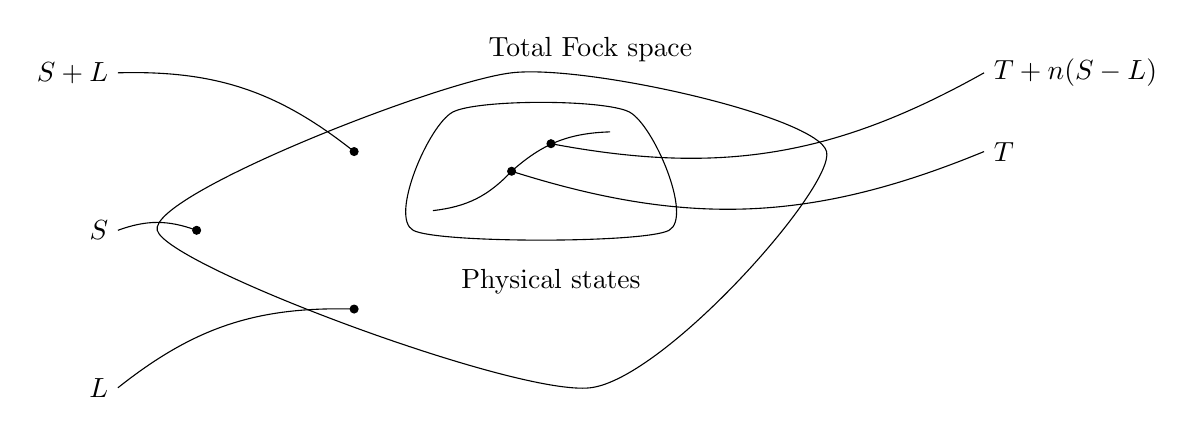
\begin{tikzpicture}
        \draw[smooth cycle, tension=0.4] plot coordinates{(2,2) (-2.5,0) (3,-2) (6,1)} node at (3,2.3) {Total Fock space};
        \draw[smooth cycle, tension=0.4] plot coordinates { (0.75, 0) (1.25, 1.5) (3.5, 1.5) (4, 0)}  node [label={[label distance=-0.3cm, xshift=-1.5cm, yshift=-0.75cm]: Physical states}] {};

        \draw[] (0, 1) to[bend right=20] (-3,2) node[left] {$\ket{S} + \ket{L}$};
        \filldraw[black] (0, 1) circle (0.05);

        \draw[] (-2, 0) to[bend right=20] (-3,0) node[left] {$\ket{S}$};
        \filldraw[black] (-2, 0) circle (0.05);

        \draw[] (0, -1) to[bend right=20] (-3,-2) node[left] {$\ket{L}$};
        \filldraw[black] (0, -1) circle (0.05);

        \draw[] (2, 0.75) to[bend right=20] (8, 1) node[right] {$\ket{T}$};
        \filldraw[black] (2, 0.75) circle (0.05);

        \draw[] (2.5, 1.1) to[bend right=20] (8, 2) node[right] {$\ket{T} + n (\ket{S} - \ket{L})$};
        \filldraw[black] (2.5,1.1) circle (0.05);

        \draw[] (1,0.25) to[bend right=20] (2, 0.75) to[bend left=20] (3.25, 1.25);

        \end{tikzpicture}
        \caption{Pictorial representation of Fock space of photons.}
        \label{fig:gauge2}
    \end{figure}

    Two states are physically equivalent if the give the same expectation value for all observables. In fact, the Hamiltonian depends only on the number of tranversal photons and the zero-norm $\ket{S} - \ket{L}$ photons are not considered at all. Therefore,given the Hamiltonian
    \begin{equation*}
        \hat H = \int \frac{d^3 p}{(2\pi)^3} |\mathbf p| ( - \hat a_{\mathbf p}^{\dagger (0)} \hat a_{\mathbf p}^{(0)} + \hat a_{\mathbf p}^{\dagger (1)} \hat a_{\mathbf p}^{(1)} + \hat a_{\mathbf p}^{\dagger (2)} \hat a_{\mathbf p}^{(2)} + \hat a_{\mathbf p}^{\dagger (3)} \hat a_{\mathbf p}^{(3)})  ~.
    \end{equation*}
    and given a physical state $\ket{\psi}$ which satisfies~\eqref{GB}, the expectation value of the hamiltonian is given only by the transversal polarisations
    \begin{equation*}
    \begin{aligned}
        \bra{\psi} \hat H \ket{\psi} & = \int \frac{d^3 p}{(2\pi)^3} |\mathbf p| ( - \cancel{\bra{\psi} \hat a_{\mathbf p}^{\dagger (0)} \hat a_{\mathbf p}^{(0)} \ket{\psi}} + \bra{\psi} \hat a_{\mathbf p}^{\dagger (1)} \hat a_{\mathbf p}^{(1)} \ket{\psi} + \bra{\psi} \hat a_{\mathbf p}^{\dagger (2)} \hat a_{\mathbf p}^{(2)} \ket{\psi} + \cancel{\bra{\psi} \hat a_{\mathbf p}^{\dagger (3)} \hat a_{\mathbf p}^{(3)} \ket{\psi}} ) \\ & = \int \frac{d^3 p}{(2\pi)^3} |\mathbf p| ( \bra{\psi} \hat a_{\mathbf p}^{\dagger (1)} \hat a_{\mathbf p}^{(1)} \ket{\psi} + \bra{\psi} \hat a_{\mathbf p}^{\dagger (2)} \hat a_{\mathbf p}^{(2)} \ket{\psi} ) = n_T |\mathbf p| ~.
    \end{aligned}
    \end{equation*}
    \begin{proof}
        The Lagrangian is
        \begin{equation*}
        \begin{aligned}
            \mathcal L & = - \frac{1}{4} F_{\mu\nu} F^{\mu\nu} - \frac{1}{2} \partial_\mu A^\mu \partial_\nu A^\nu = - \frac{1}{4} (\partial_\mu A_\nu - \partial_\nu A_\mu) (\partial^\mu A^\nu - \partial^\nu A^\mu) - \frac{1}{2} \partial_\mu A^\mu \partial_\nu A^\nu \\ & = - \frac{1}{4} \partial_\mu A_\nu \partial^\mu A^\nu + \frac{1}{4} \partial_\mu A_\nu \partial^\nu A^\mu + \frac{1}{4} \partial_\nu A_\mu \partial^\mu A^\nu - \frac{1}{4} \partial_\nu A_\mu \partial^\nu A^\mu - \frac{1}{2} \partial_\mu A^\mu \partial_\nu A^\nu \\ & = - \frac{1}{2} \partial_\mu A_\nu \partial^\mu A^\nu + \frac{1}{2} \underbrace{(\partial_\mu A_\nu \partial^\nu A^\mu - \partial_\mu A^\mu \partial_\nu A^\nu) }_{ - A_\nu  \partial_\mu \partial^\nu A^\mu - A^\mu \partial_\mu \partial_\nu A^\nu + \textnormal{boundary terms}} \\ & = - \frac{1}{2} \partial_\mu A_\nu \partial^\mu A^\nu + \frac{1}{2} (- A_\nu  \partial_\mu \partial^\nu A^\mu - A^\mu \partial_\mu \partial_\nu A^\nu) \\ & = - \frac{1}{2} \partial_\mu A_\nu \partial^\mu A^\nu + \frac{1}{2} (- \cancel{A_\mu  \partial_\nu \partial^\mu A^\nu} + \cancel{A^\mu \partial_\nu \partial_\mu A^\nu}) = - \frac{1}{2} \partial_\mu A_\nu \partial^\mu A^\nu ~,
        \end{aligned}
        \end{equation*}
        where we have integrated by parts since the Lagrangian is always integrated to obtain the action. The conjugate field is 
        \begin{equation*}
            \pi^\mu = \pdv{\mathcal L}{\dot A_\mu} = - \dot A_\mu ~.
        \end{equation*}
        The Hamiltonian is 
        \begin{equation*}
        \begin{aligned}
            \mathcal H & = \pi^\mu \underbrace{\dot A_\mu}_{- \pi_\mu} - \mathcal L = - \pi^\mu \pi_\mu + \frac{1}{2} \partial_\mu A_\nu \partial^\mu A^\nu \\ & = - \pi^\mu \pi_\mu + \frac{1}{2} \underbrace{\dot A^\mu \dot A_\mu}_{\pi^\mu \pi_\mu} + \frac{1}{2} \partial_i A_\mu \partial^i A^\mu = - \frac{1}{2} \pi^\mu \pi_\mu + \frac{1}{2} \partial_i A_\mu \partial^i A^\mu = \mathcal H_1 + \mathcal H_2 ~.
        \end{aligned}
        \end{equation*}
        Now, we promote to operator. 
        \begin{equation*}
            \hat H = \int d^3 x ~ \mathcal H ~.
        \end{equation*}
        The first part is 
        \begin{equation*}
        \begin{aligned}
            & \hat H_1 = - \frac{1}{2} \int d^3 x ~ \hat \pi^\mu \hat \pi_\mu \\ & = - \frac{1}{2} \int d^3 x \int \frac{d^3 p}{(2\pi)^3} i \sqrt{\frac{|\mathbf p|}{2}} \sum_{\lambda=0}^{3} \epsilon^{\mu(\lambda)} (\mathbf p) \Big ( \hat a_{\mathbf p}^{(\lambda)}   \exp(i \mathbf p \cdot \mathbf x) - \hat a_{\mathbf p}^{\dagger (\lambda)}   \exp(- i \mathbf p \cdot \mathbf x) \Big) \\ & \quad \int \frac{d^3 q}{(2\pi)^3} i \sqrt{\frac{|\mathbf q|}{2}} \sum_{\lambda'=0}^{3} \epsilon_{\mu(\lambda')} (\mathbf q)  \Big ( \hat a_{\mathbf q}^{(\lambda')}   \exp(i \mathbf q \cdot \mathbf x) - \hat a_{\mathbf q}^{\dagger (\lambda')}   \exp(- i \mathbf q \cdot \mathbf x) \Big) \\ & = \frac{1}{4} \int \frac{d^3 x ~ d^3 p ~ d^3 q}{(2\pi)^6} \sqrt{|\mathbf p| |\mathbf q|} \sum_{\lambda=0}^{3} \sum_{\lambda'=0}^{3} \underbrace{\epsilon^{\mu(\lambda)} (\mathbf p) \epsilon_{\mu(\lambda')} (\mathbf q)}_{\eta^{\lambda \lambda'}} ( \hat a_{\mathbf p}^{(\lambda)}   \hat a_{\mathbf q}^{(\lambda')}   \underbrace{\exp(i  \mathbf x \cdot (\mathbf p + \mathbf q)) }_{\delta(\mathbf p + \mathbf q)}  \\ & \quad - \hat a_{\mathbf p}^{(\lambda)}  \hat a_{\mathbf q}^{\dagger (\lambda')}   \underbrace{\exp(i  \mathbf x \cdot (\mathbf p - \mathbf q)) }_{\delta(\mathbf p - \mathbf q)} - \hat a_{\mathbf p}^{\dagger (\lambda)}   \hat a_{\mathbf q}^{(\lambda')}   \underbrace{\exp(i  \mathbf x \cdot (- \mathbf p + \mathbf q)) }_{\delta(\mathbf p - \mathbf q)} \\ & \quad + \hat a_{\mathbf p}^{\dagger (\lambda)}   \hat a_{\mathbf q}^{\dagger (\lambda')}   \underbrace{\exp(- i  \mathbf x \cdot (\mathbf p + \mathbf q)) }_{\delta(\mathbf p + \mathbf q)} )
        \end{aligned}
        \end{equation*}
        \begin{equation*}
        \begin{aligned}
            & = \frac{1}{4} \int \frac{d^3 x}{(2\pi)^3} |\mathbf p| \sum_{\lambda=0}^{3} \sum_{\lambda'=0}^{3} \eta^{\lambda \lambda'} ( \hat a_{\mathbf p}^{(\lambda)} \hat a_{- \mathbf p}^{(\lambda')}  - \hat a_{\mathbf p}^{(\lambda)} \hat a_{\mathbf p}^{\dagger (\lambda')}  - \hat a_{\mathbf p}^{\dagger (\lambda)} \hat a_{\mathbf p}^{(\lambda')} + \hat a_{\mathbf p}^{\dagger (\lambda)} \hat a_{- \mathbf p}^{\dagger (\lambda')} ) ~.
        \end{aligned}
        \end{equation*}
        Given 
        \begin{equation*}
            \partial_i \hat A_\mu = \int \frac{d^3 p}{(2\pi)^3} \frac{1}{\sqrt{2 |\mathbf p|}} \sum_{\lambda=0}^{3} \epsilon_\mu^{(\lambda)} (\mathbf p) \Big ( (- i p_i )\hat a_{\mathbf p}^{(\lambda)} \exp(i \mathbf p \cdot \mathbf x) + (i p_i)\hat a_{\mathbf p}^{\dagger (\lambda)}  \exp(- i \mathbf p \cdot \mathbf x) \Big) ~,
        \end{equation*}
        the second part is
        \begin{equation*}
        \begin{aligned}
            & \hat H_2 = \frac{1}{2} \int d^3 x ~ \partial_i \hat A_\mu \partial^i \hat A^\mu \\ & = \frac{1}{2} \int d^3 x \int \frac{d^3 p}{(2\pi)^3} \frac{1}{\sqrt{2 |\mathbf p|}} \sum_{\lambda=0}^{3} \epsilon_\mu^{(\lambda)} (\mathbf p) \Big ( (- i p_i ) \hat a_{\mathbf p}^{(\lambda)} \exp(i \mathbf p \cdot \mathbf x) + (i p_i)\hat a_{\mathbf p}^{\dagger (\lambda)}  \exp(- i \mathbf p \cdot \mathbf x) \Big) \\ & \quad \int \frac{d^3 q}{(2\pi)^3} \frac{1}{\sqrt{2 |\mathbf q}} \sum_{\lambda'=0}^{3} \epsilon^{\mu(\lambda')} (\mathbf q) \Big ( (- i q^i )\hat a_{\mathbf q}^{(\lambda')} \exp(i \mathbf q \cdot \mathbf x) + (i q^i)\hat a_{\mathbf q}^{\dagger (\lambda')} \exp(- i \mathbf q \cdot \mathbf x) \Big) \\ & = \frac{1}{2} \int \frac{d^3 x ~ d^3 p ~ d^3 q}{(2\pi)^6} \frac{1}{2\sqrt{|\mathbf p| |\mathbf q|}} \sum_{\lambda=0}^{3} \sum_{\lambda'=0}^{3} \underbrace{\epsilon^{\mu(\lambda)} (\mathbf p) \epsilon_{\mu}^{(\lambda')} (\mathbf q)}_{\eta^{\lambda \lambda'}} p_i q^i ( \hat a_{\mathbf p}^{(\lambda)} \hat a_{\mathbf q}^{(\lambda)} \underbrace{\exp(i  \mathbf x \cdot (\mathbf p + \mathbf q)) }_{\delta(\mathbf p + \mathbf q)} \\ & \quad - \hat a_{\mathbf p}^{(\lambda)}\hat a_{\mathbf q}^{\dagger (\lambda)} \underbrace{\exp(i \mathbf x \cdot (\mathbf p - \mathbf q)) }_{\delta(\mathbf p - \mathbf q)} - \hat a_{\mathbf p}^{\dagger (\lambda)} \hat a_{\mathbf q}^{(\lambda)} \underbrace{\exp( i  \mathbf x \cdot ( -\mathbf p + \mathbf q)) }_{\delta(\mathbf p - \mathbf q)} \\ & \quad + \hat a_{\mathbf p}^{\dagger (\lambda)} \hat a_{\mathbf q}^{\dagger (\lambda)} \underbrace{\exp(- i  \mathbf x \cdot (\mathbf p + \mathbf q)) }_{\delta(\mathbf p + \mathbf q)})
        \end{aligned}
        \end{equation*}
        \begin{equation*}
        \begin{aligned}
            & = \frac{1}{2} \int \frac{d^3 p}{(2\pi)^3} \frac{1}{2 |\mathbf p|} \sum_{\lambda=0}^{3} \sum_{\lambda'=0}^{3} \eta^{\lambda \lambda'} |\mathbf p|^2 (- \hat a_{\mathbf p}^{(\lambda)} \hat a_{- \mathbf p}^{(\lambda')} - \hat a_{\mathbf p}^{(\lambda)} \hat a_{\mathbf p}^{\dagger (\lambda')} - \hat a_{\mathbf p}^{\dagger (\lambda)} \hat a_{\mathbf p}^{(\lambda')} - \hat a_{\mathbf p}^{\dagger (\lambda)} \hat a_{-\mathbf p}^{\dagger (\lambda')} ) \\ & = \frac{1}{4} \int \frac{d^3 p}{(2\pi)^3} |\mathbf p| \sum_{\lambda=0}^{3} \sum_{\lambda'=0}^{3} \eta^{\lambda \lambda'} (- \hat a_{\mathbf p}^{(\lambda)} \hat a_{- \mathbf p}^{(\lambda')} - \hat a_{\mathbf p}^{(\lambda)} \hat a_{\mathbf p}^{\dagger (\lambda')} - \hat a_{\mathbf p}^{\dagger (\lambda)} \hat a_{\mathbf p}^{(\lambda')} - \hat a_{\mathbf p}^{\dagger (\lambda)} \hat a_{-\mathbf p}^{\dagger (\lambda')} ) ~.
        \end{aligned}
        \end{equation*}
        Putting everything together 
        \begin{equation*}
        \begin{aligned}
            \hat H & = \frac{1}{4} \int \frac{d^3 p}{(2\pi)^3} |\mathbf p| \sum_{\lambda=0}^{3} \sum_{\lambda'=0}^{3} \eta^{\lambda \lambda'} (- \cancel{\hat a_{\mathbf p}^{(\lambda)} \hat a_{- \mathbf p}^{(\lambda')}} - \hat a_{\mathbf p}^{(\lambda)} \hat a_{\mathbf p}^{\dagger (\lambda')} - \hat a_{\mathbf p}^{\dagger (\lambda)} \hat a_{\mathbf p}^{(\lambda')} - \cancel{\hat a_{\mathbf p}^{\dagger (\lambda)} \hat a_{-\mathbf p}^{\dagger (\lambda')}} ) \\ & \quad + \frac{1}{4} \int \frac{d^3 x}{(2\pi)^3} |\mathbf p| \sum_{\lambda=0}^{3} \sum_{\lambda'=0}^{3} \eta^{\lambda \lambda'} ( \cancel{\hat a_{\mathbf p}^{(\lambda)} \hat a_{- \mathbf p}^{(\lambda')}}  - \hat a_{\mathbf p}^{(\lambda)} \hat a_{\mathbf p}^{\dagger (\lambda')}  - \hat a_{\mathbf p}^{\dagger (\lambda)} \hat a_{\mathbf p}^{(\lambda')} + \cancel{\hat a_{\mathbf p}^{\dagger (\lambda)} \hat a_{- \mathbf p}^{\dagger (\lambda')}} ) \\ & = \frac{1}{2} \int \frac{d^3 p}{(2\pi)^3} |\mathbf p| \sum_{\lambda=0}^{3} \sum_{\lambda'=0}^{3} \eta^{\lambda \lambda'} (- \hat a_{\mathbf p}^{(\lambda)} \hat a_{\mathbf p}^{\dagger (\lambda')} - \hat a_{\mathbf p}^{\dagger (\lambda)} \hat a_{\mathbf p}^{(\lambda')})
        \end{aligned}
        \end{equation*}
        which in normal ordering is 
        \begin{equation*}
        \begin{aligned}
            \hat H & = \int \frac{d^3 p}{(2\pi)^3} |\mathbf p| \sum_{\lambda=0}^{3} \sum_{\lambda'=0}^{3} \eta^{\lambda \lambda'} (- \hat a_{\mathbf p}^{\dagger (\lambda)} \hat a_{\mathbf p}^{(\lambda')}) \\ & = \int \frac{d^3 p}{(2\pi)^3} |\mathbf p| \sum_{\lambda=0}^{3} (- \hat a_{\mathbf p}^{\dagger (0)} \hat a_{\mathbf p}^{(0)} + \hat a_{\mathbf p}^{\dagger (1)} \hat a_{\mathbf p}^{(1)} + \hat a_{\mathbf p}^{\dagger (2)} \hat a_{\mathbf p}^{(2)}+ \hat a_{\mathbf p}^{\dagger (3)} \hat a_{\mathbf p}^{(3)}) ~.
        \end{aligned}
        \end{equation*}
    \end{proof}

    To summarise, any observables gives only results in terms of transversal photons and gauge equivalent states are all physically equivalent, since they are indistinguishable in measurements of observables. The only truly physical degrees of freedome of a massless spin-$1$ particle described by the Maxwell's field are the two transversal polarisations. However, this is not true for massive photons, since the longitudinal polararisation is the thire degree of freedom.

\section{Massive photons}    

    Massive photons are described by the Proca lagrangian
    \begin{equation*}
        \mathcal L = - \frac{1}{4} F^{\mu\nu} F_{\mu\nu} - \frac{m^2}{2} A_\mu A^\mu ~,
    \end{equation*}
    where the equations of motion are 
    \begin{equation*}
        \partial_\mu F^{\mu\nu} + m^2 A^\nu = 0~.
    \end{equation*}
    Notice that the Lorenz gauge is automatically always satisfied and it is not imposed by hand.
    \begin{proof}
        In fact, we have
        \begin{equation}
            0 = \underbrace{\partial_\mu \partial_\nu}_{\text{symm}} \underbrace{F^{\mu\nu}}_{\text{anti}} + m^2 \partial_\nu A^\nu = m^2 \partial_\nu A^\nu ~.
        \end{equation}
    \end{proof}
    The equations of motion become
    \begin{equation*}
        (\Box + m^2) A^\mu (x) = 0 ~.
    \end{equation*}
    \begin{proof}
        In fact, we have
        \begin{equation*}
            0 = \partial_\mu F^{\mu\nu} + m^2 A^\nu = \partial_\mu \partial^\mu A^\nu - \cancel{\partial_\mu \partial^\nu A^\nu} + m^2 A^\nu = (\Box + m^2) A^\nu ~.
        \end{equation*}
    \end{proof}
    Therefore, each $A^\mu$ satisfies the Klein-Gordon equation but there are only $3$ independent degrees of freedom by the Lorenz gauge. Finally, notice that the mass term breaks the gauge symmetry, since for a gauge transformation ${A'}_\mu = A_\mu + \partial_\mu \lambda$
    \begin{equation*}
        \frac{m}{2} {A'}^\mu {A'}_\mu \neq \frac{m}{2} A^\mu A_\mu ~.
    \end{equation*}
